% step_5a_factorial -- 2x2 (bandwidth x reg) factorial isolating the 5a velocity collapse
% Build:  pdflatex step_5a_factorial.tex
\documentclass[10pt,a4paper]{article}
\usepackage[T1]{fontenc}\usepackage[utf8]{inputenc}\usepackage{charter}
\usepackage[scaled=0.88]{helvet}\usepackage{amsmath}\usepackage{amssymb}
\usepackage[margin=1.55cm,top=1.25cm,bottom=1.0cm]{geometry}
\usepackage{xcolor}\usepackage{titlesec}\usepackage{enumitem}\usepackage{microtype}\usepackage{parskip}
\usepackage{graphicx}
\renewcommand{\baselinestretch}{0.97}\setlength{\parskip}{2.3pt}\pagestyle{empty}\raggedbottom
\definecolor{acc}{HTML}{1B4F72}\definecolor{gry}{HTML}{555555}
\titleformat{\section}{\sffamily\bfseries\footnotesize\color{acc}}{\thesection.}{0.4em}{\MakeUppercase}
\titlespacing{\section}{0pt}{5pt}{1.5pt}
\newcommand{\co}[1]{{\small\texttt{#1}}}
\setlist[itemize]{leftmargin=1.05em,itemsep=1.0pt,topsep=1.2pt,parsep=0pt}
\begin{document}\small

{\sffamily\bfseries\large\color{acc} cloudtorch / develop\, --- Step 5a: the velocity collapse is the regularisation}

\vspace{1pt}
{\sffamily\color{gry}\footnotesize 2026-08-24 --- controlled 2$\times$2 factorial isolating why 4a's velocity maps have structure and 5a's collapse. \textbf{Corrects} \co{step\_5a\_debug.pdf}: the earlier note concluded ``the real lever is \emph{not} a reg knob.'' That was wrong --- the explicit regularisation is exactly the lever.}

\vspace{1pt}{\footnotesize\color{gry}\rule{\textwidth}{0.4pt}}

%% ------------------------------------------------
\section{What was run}

A clean 2$\times$2 on \textbf{fixed frames} [11--14] (4a's window), the \textbf{committed} \co{pinn\_model.py} init ($v_{\rm los}\!=\!\mp20$, scale 20 --- what produced the stored 4a/5a outputs, restored by monkeypatch), and every other knob held constant (\co{N\_FREQ}=256, \co{SIGMA\_T}=4, \co{WIDTH}=256, \co{DEPTH}=4, \co{S\_MAX}=0.7, \co{DV\_FLOOR}=8, \co{LR}=3e-3, 3000 iters, seed 0). \textbf{Only two things vary:}
\begin{itemize}
\item \co{SIGMA\_XY} $\in\{12,\,32\}$ --- the Fourier spatial bandwidth (implicit smoothness);
\item regularisation $\in\{$off (4a), on (5a's original \co{REG}, \co{w\_xy}=1e-3)$\}$.
\end{itemize}
Runs: A=(32,\,off)\,$\approx$\,4a, B=(12,\,off), C=(32,\,on), D=(12,\,on)\,$\approx$\,5a. Script: \co{scratchpad/ab\_4a\_vs\_5a.py}.

%% ------------------------------------------------
\section{Result}

\begin{center}\small
\begin{tabular}{llccl l}
\hline
run & \co{SIGMA\_XY} / reg & $\langle\chi^2\rangle$ & RMS & $v_{1}$ [min/med/max] & $v_{2}$ [min/med/max]\\
\hline
A & 32 / \textbf{off} & 0.252 & 3.96\% & $-226/{-}17/\mathbf{+52}$ & $-308/{-}56/{-}10$\\
B & 12 / \textbf{off} & 0.195 & 3.48\% & $-96/{-}16/\mathbf{+51}$  & $-183/{-}54/\mathbf{+24}$\\
C & 32 / \textbf{on}  & 0.604 & 6.13\% & $-71/{-}27/\mathbf{-27}$  & $+18/{+}25/\mathbf{+25}$\\
D & 12 / \textbf{on}  & 0.904 & 7.50\% & $-47/{-}21/\mathbf{-21}$  & $-13/{-}12/{+}4$\\
\hline
\end{tabular}
\end{center}

Read the last two columns: reg \textbf{off} $\Rightarrow$ velocities span a wide, \emph{sign-crossing} range (structure); reg \textbf{on} $\Rightarrow$ min\,$\approx$\,med\,$\approx$\,max (a single collapsed value). This holds at \emph{both} bandwidths.

%% ------------------------------------------------
\section{Finding: reg decides collapse; bandwidth does not}

Toggling the regularisation flips structured\,$\leftrightarrow$\,collapsed at either \co{SIGMA\_XY}; changing \co{SIGMA\_XY} at fixed reg does \emph{not}. So \co{SIGMA\_XY} only sets how rough the maps get (higher $=$ wilder tails: $v_1$ reaches $-226$ in A vs $-96$ in B); the \textbf{explicit regularisation is what collapses the velocity field}. As a bonus the reg also \emph{worsens} the data fit here ($\chi^2$ $0.2\!\to\!0.6$--$0.9$).

\begin{center}
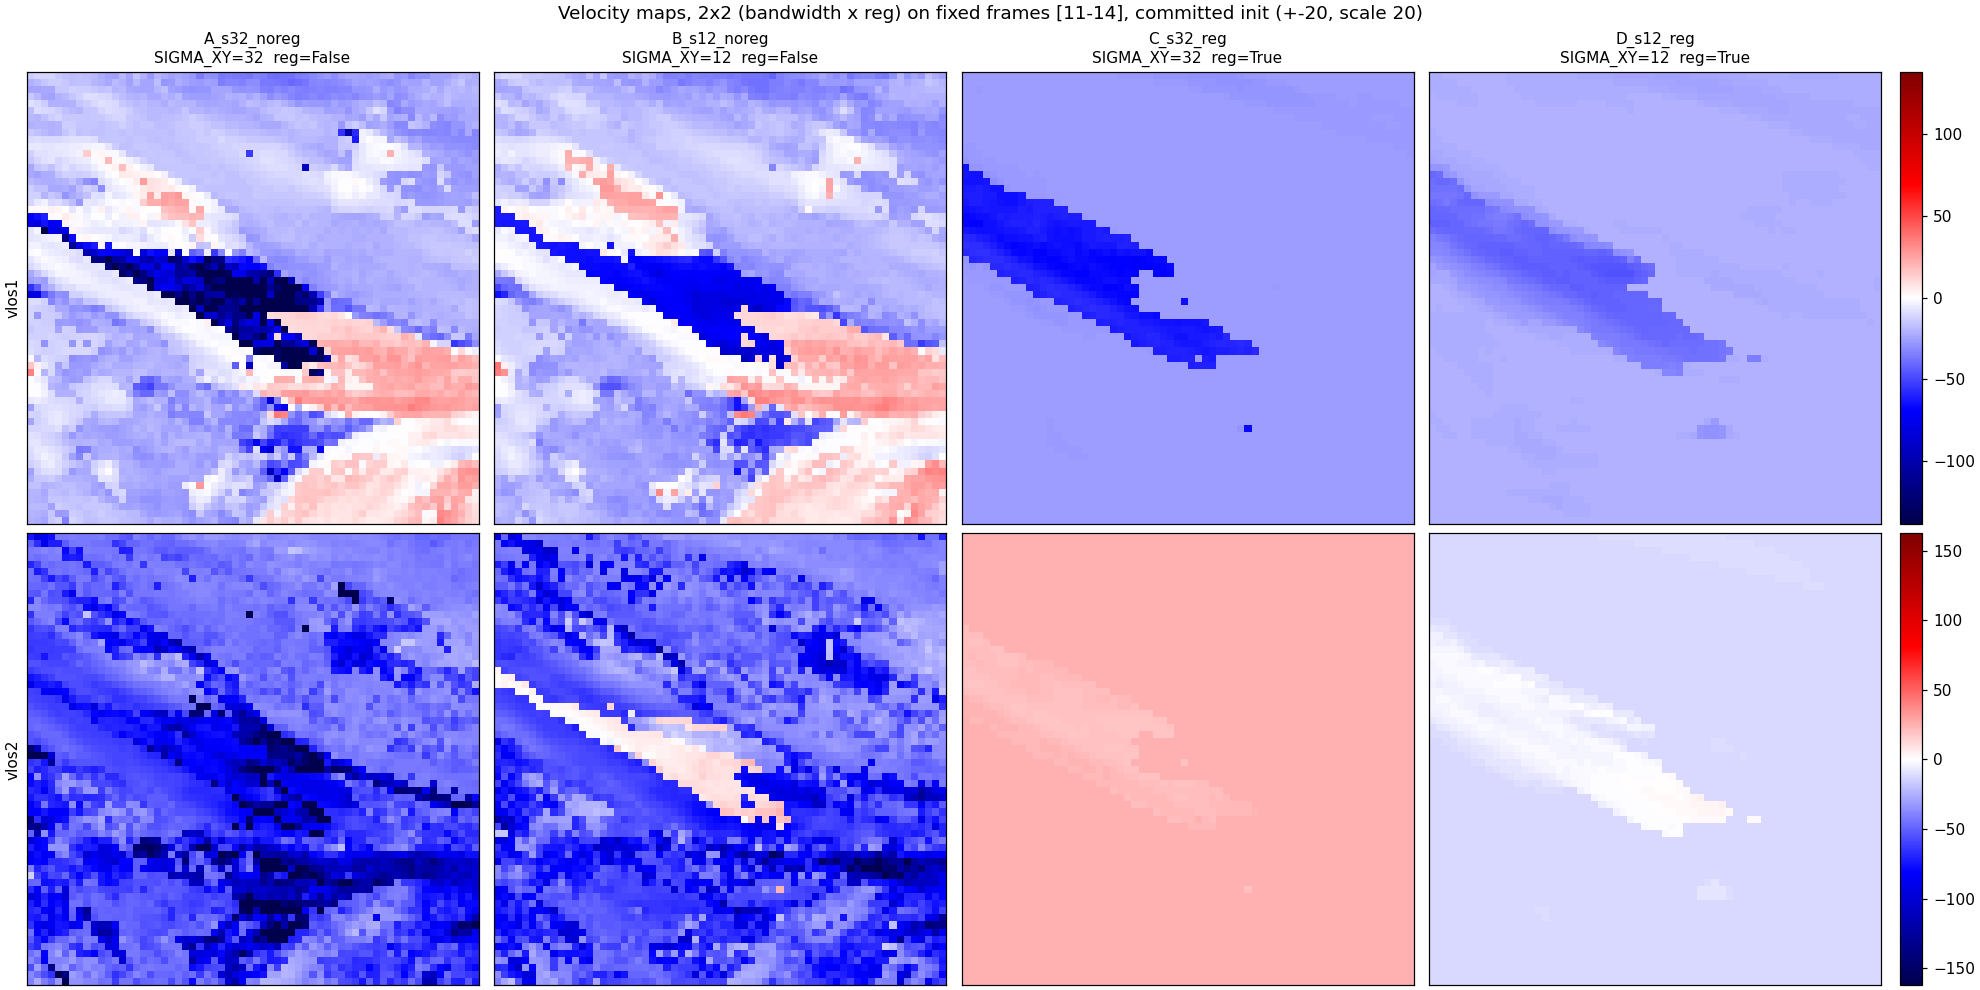
\includegraphics[width=0.98\textwidth]{step_5a_factorial_vlos.png}
\end{center}
\vspace{-4pt}
{\footnotesize\color{gry} $v_{\rm los1}$ (top) and $v_{\rm los2}$ (bottom) for the four runs, common colour scale per row. Reg-off (A,\,B): filamentary, sign-crossing flows. Reg-on (C,\,D): near-uniform.}

%% ------------------------------------------------
\section{Why a $\sim$1--2\% penalty dominates (and why the earlier fix missed)}

The reg is only \textbf{0.8--2.0\%} of the loss yet flattens the velocity completely, because $v_{\rm los}$ is a \emph{near-flat, weakly-constrained} direction: the given background owns the line wings where the Doppler signal lives, so the data barely pulls on velocity. A tiny smoothness/hinge penalty then dominates that null direction and pulls the whole field to a constant. ``Non-binding in loss magnitude'' $\ne$ ``harmless.'' This also explains why relaxing \textbf{only} \co{w\_xy} $100\times$ (the \co{step\_5a\_debug} test) didn't help: it left the \emph{other} velocity terms --- temporal \co{w\_t}=2e-3 and the \co{vlos} range hinge --- active, and \emph{those} drive the collapse.

%% ------------------------------------------------
\section{Next levers}

\begin{itemize}
\item \textbf{Cut the velocity reg as a whole} (\co{w\_t} $+$ hinge, not \co{w\_xy} alone), $\sim$10--100$\times$ weaker, until structure survives while $\chi^2$ stays low.
\item \textbf{Sub-factorial} (\co{w\_t}-only / hinge-only / \co{w\_xy}-only) to pin down which term dominates --- not yet isolated.
\item Reg-off carries unphysical tails ($v_1\!\to\!-226$, \co{dv1}$\to$151): the aim is a penalty that \emph{clips outliers without flattening} (robust loss or a far-outer hinge), not the current over-scaled velocity smoothing.
\end{itemize}

\vspace{1pt}{\footnotesize\color{gry}\rule{\textwidth}{0.4pt}}
{\sffamily\color{gry}\footnotesize Runs used the \emph{committed} \co{pinn\_model.py} ($\mp20$, scale 20). The working tree now carries an uncommitted asymmetric init ($-50/0$, scale 5), so neither notebook's stored output reproduces as-is. Figure: \co{docs/step\_5a\_factorial\_vlos.png}.}

\end{document}
